\chapter[Solución propuesta]{Solución Propuesta} \label{sec:solucion_propuesta}
A partir del marco teórico desarrollado en los capítulos anteriores, en particular del análisis de acopladores direccionales del Capítulo~\ref{cp:introduction}, de los criterios de diseño de amplificadores de potencia discutidos en el Capítulo~\ref{sec:teoria_pa} y del análisis comparativo de tecnologías semiconductoras del Capítulo~\ref{sec:gan_hemt} se desarrollaron dos circuitos de radiofrecuencia para el subsistema de comunicaciones en banda S de la misión CubeSat, un acoplador híbrido en cuadratura y un amplificador de potencia monoetapa basado en el transistor GaN HEMT CGH40006S~\cite{macom}, polarizado en Clase AB.

De acuerdo con el Reglamento de Radiocomunicaciones de la Unión Internacional de Telecomunicaciones \cite{itu2024}, el rango de 2170~MHz a 2200~MHz se asigna al Servicio Móvil por Satélite (MSS) para enlaces de bajada, mientras que el intervalo de 2200~MHz a 2290~MHz se destina a la investigación espacial. Operar en torno a 2200~MHz resulta provechoso al encontrarse en la proximidad de ambas bandas, lo que permite mantener compatibilidad espectral con sistemas MSS y a su vez alinearse con las frecuencias utilizadas en misiones de exploración e investigación espacial. Por este motivo, se estableció la frecuencia de portadora de 2,2~GHz como frecuencia de operación tanto del acoplador como del amplificador desarrollados.

El desarrollo de ambos circuitos siguió una misma metodología de trabajo, estructurada en tres etapas sucesivas, a saber, el diseño y la simulación del circuito empleando un software especializado, el diseño del circuito impreso correspondiente y su fabricación, y la caracterización experimental del prototipo resultante mediante un conjunto de mediciones de laboratorio. Dado que esta metodología resulta común a ambos desarrollos, con la salvedad de las particularidades propias del comportamiento pasivo del acoplador frente al comportamiento activo y no lineal del amplificador, se la describe de manera conjunta en las secciones siguientes, antes de abordar el proceso de diseño específico de cada circuito.

Las Secciones~\ref{sec:diseno_acoplador} y~\ref{sec:diseno_amplificador} desarrollan, respectivamente, el diseño del acoplador híbrido y el diseño del amplificador de potencia, incluyendo en este último caso el análisis de radioenlace satelital que determinó la potencia de salida y el esquema de modulación objetivo de la misión. Los resultados de la caracterización experimental de ambos prototipos se presentan en el Capítulo~\ref{sec:resultados}.

% -----------------------------------------------------------------------------------------------%
\section{Metodología de diseño y simulación} \label{sec:metodologia_diseno_sim}
El diseño y la simulación de ambos circuitos se realizaron mediante el entorno Advanced Design System (ADS) de Keysight, empleando bibliotecas de modelos para componentes reales de montaje superficial (SMD) provista por los fabricantes correspondientes, en lugar de modelos ideales de elementos discretos. Sobre el esquemático de simulación de cada circuito se ejecutaron rutinas de optimización numérica para ajustar las dimensiones de las líneas de transmisión que conforman las redes de adaptación y de acoplamiento, hasta alcanzar las condiciones de desempeño requeridas en la frecuencia de operación. Adicionalmente, en los casos en que el circuito requería capacitores o inductores discretos, se realizó una optimización sobre el valor de dichos componentes, en la cual el optimizador recorrió el conjunto de valores disponibles en la biblioteca de componentes reales para el capacitor o el inductor correspondiente, en lugar de optimizar un valor continuo de capacitancia o inductancia sin restricción, de modo de obtener directamente un diseño realizable.

Adicionalmente, en el caso particular del acoplador, se empleó simulación electromagnética de onda completa para verificar el comportamiento del layout de PCB una vez finalizado su diseño, mediante los entornos High Frequency Structure Simulator (HFSS) de Ansys y CST Studio Suite de Dassault Systèmes~\cite{cst}. Ambas herramientas se emplearon de manera comparativa entre sí, mientras que los resultados obtenidos en CST fueron los adoptados como referencia para la comparación con las mediciones experimentales presentada en el Capítulo~\ref{sec:resultados}.

El conjunto específico de simulaciones realizadas sobre cada circuito difirió de acuerdo con su naturaleza. En el caso del acoplador, un circuito pasivo y lineal, la caracterización se realizó fundamentalmente mediante la simulación de parámetros S a nivel de esquemático y mediante la simulación electromagnética de onda completa del layout descripta en el párrafo anterior. En el caso del amplificador, un circuito activo y no lineal, se incorporaron en cambio simulaciones de estabilidad, de load-pull, de balance armónico y de transitorio en el dominio temporal, orientadas a caracterizar su comportamiento de gran señal, sin recurrir a simulación electromagnética de onda completa. Estas simulaciones adicionales, así como su fundamento, se describen en la Sección~\ref{sec:diseno_amplificador}.

% -----------------------------------------------------------------------------------------------%
\section{Metodología de diseño de PCB} \label{sec:metodologia_pcb}
El diseño del circuito impreso (PCB) de ambos desarrollos se realizó en el entorno Altium Designer, a partir de los modelos de las líneas de transmisión previamente dimensionadas y optimizadas en ADS, los cuales se exportaron y trasladaron al layout de la placa. Sobre dicho layout se incorporaron las vías de masa requeridas para garantizar la continuidad del plano de referencia y se configuró la estructura de capas (stackup) de la placa de acuerdo con el proceso de fabricación JLC04161H-7628 del fabricante JLCPCB, una estructura de cuatro capas en sustrato FR4, empleada de manera común para ambos circuitos. La elección de este proceso específico se fundamentó en que ofrece impedancia controlada de $50\,\Omega$ como servicio estándar del fabricante, y en que había sido previamente empleado en proyectos previos con buenos resultados, lo cual permitió reutilizar parámetros de diseño y de fabricación ya validados experimentalmente con anterioridad. La Tabla~\ref{tab:pcb_stackup} detalla la estructura de capas resultante.

\begin{table}[b]
    \caption{PCB Stackup}
    \label{tab:pcb_stackup}
    \centering
    \renewcommand{\arraystretch}{1.1}
    \begin{tabular}{|l|c|c|}
        \hline
        \textbf{Capa} & \textbf{Permitividad Relativa (Dk)} & \textbf{Espesor} \\
        \hline
        Top      & \cellcolor{coppercolor}Copper  & 0.035mm   \\ \hline
        Prepreg  & \cellcolor{dielectriccolor}4.4 & 0.21040mm \\ \hline
        Inner L2 & \cellcolor{coppercolor}Copper  & 0.0152mm  \\ \hline
        Core     & \cellcolor{dielectriccolor}4.6 & 1.065mm   \\ \hline
        Inner L3 & \cellcolor{coppercolor}Copper  & 0.0152mm  \\ \hline
        Prepreg  & \cellcolor{dielectriccolor}4.4 & 0.21040mm \\ \hline
        Bottom   & \cellcolor{coppercolor}Copper  & 0.035mm   \\
        \hline
    \end{tabular}
\end{table}

El diseño del layout de RF incorporó un conjunto de criterios y prácticas recomendadas, comunes a ambos circuitos, para minimizar las pérdidas y las desadaptaciones parásitas inherentes a la implementación física del diseño:

\begin{itemize}
    \item Los caminos de señal de radiofrecuencia se trazaron de la forma más rectilínea posible, evitando curvas y quiebres innecesarios que pudieran introducir desadaptaciones de impedancia.
    \item La separación entre pistas de señal, y entre pistas y el plano de masa adyacente, se estableció en al menos cinco veces el espesor del dieléctrico correspondiente, con el objetivo de evitar acoplamiento electromagnético indeseado entre conductores próximos.
    \item Las distancias entre vías de masa se mantuvieron por debajo de $\lambda/10$ en la frecuencia de operación, con el objetivo de evitar la aparición de acoplamiento parásito entre vías adyacentes, y se emplearon múltiples vías en paralelo en los puntos críticos de conexión a masa con el fin de reducir la inductancia parásita asociada.
    \item Se prestó especial atención al acople de masa de los conectores SMA, cuyo estándar de conexión exige un acople de masa adecuado para garantizar la continuidad de la referencia entre el conector y la placa.
    \item Las líneas de transmisión que no requerían un valor de impedancia específico para el funcionamiento del circuito se diseñaron con impedancia característica de $50\,\Omega$, manteniendo consistencia con la impedancia de referencia del sistema y de los instrumentos de medición.
\end{itemize}

Adicionalmente, en el caso particular del amplificador se procuró un correcto acople de masa en zonas críticas del layout, en particular en la masa del transistor, además de la masa de los conectores SMA ya mencionada entre los criterios generales. El orden de montaje de los capacitores de filtrado de las fuentes de polarización se estableció de acuerdo con su valor de capacitancia, ubicando el capacitor de mayor valor más próximo a la fuente de alimentación, dado que su frecuencia de autorresonancia resulta más baja que la de los capacitores de menor valor, los cuales se ubicaron progresivamente más cerca del transistor para filtrar las componentes de mayor frecuencia. Estas y otras consideraciones específicas del layout de cada circuito se detallan en las respectivas secciones de diseño

Respecto del montaje de los componentes sobre la placa fabricada, los componentes SMD de la placa del amplificador de potencia fueron soldados por la empresa de montaje Outsource, dada la precisión requerida por los componentes de menor tamaño y por el propio transistor de potencia. Los conectores SMA de ambas placas, en cambio, fueron soldados manualmente por los integrantes del grupo.

% -----------------------------------------------------------------------------------------------%
\section{Metodología de medición} \label{sec:metodologia_medicion}
Para validar experimentalmente el diseño propuesto, se llevó a cabo un conjunto de mediciones sobre ambos prototipos fabricados. Estas mediciones se realizaron con la colaboración del Dr.~Ing.~Manuel García, en la Comisión Nacional de Energía Atómica (CNEA), y del Ing.~Sanca, en la Universidad Nacional de San Martín (UNSAM). Cada medición requirió un setup dedicado, descrito en las subsecciones siguientes, agrupadas de acuerdo con el circuito bajo prueba.

\subsection{Mediciones del acoplador}
Dado su comportamiento pasivo y lineal, la caracterización experimental del acoplador se limitó a la medición de sus parámetros de dispersión. Al tratarse de un circuito pasivo, no fue necesario incorporar atenuadores de protección a la salida.

Esta caracterización se llevó a cabo en dos instancias. En una primera instancia, se realizó una medición preliminar en la facultad, con un VNA FieldFox N9917A de Keysight~\cite{fieldfox} y la asistencia del Dr.~Ing.~Matías Hampel, con el único objetivo de corroborar el funcionamiento correcto del prototipo antes de proceder a su caracterización definitiva. En una segunda instancia, se realizó la medición definitiva en CNEA, empleando un analizador de redes vectorial (VNA) Keysight N5242B PNA-X~\cite{pnax}. Si bien dicho instrumento dispone de cuatro puertos, la calibración se realizó únicamente a dos puertos mediante el método TOSM, dado que la calibración a cuatro puertos requiere un tiempo considerablemente mayor que no resultaba compatible con la disponibilidad horaria de uso del equipo. En consecuencia, la matriz de dispersión completa del acoplador se obtuvo iterando las conexiones de los puertos de entrada y salida del dispositivo bajo prueba entre las dos calibraciones de puerto disponibles del instrumento.

% TODO: confirmar rango de frecuencias efectivamente barrido y nivel de potencia empleado en ambas mediciones.
\begin{figure}[H]
    \centering
    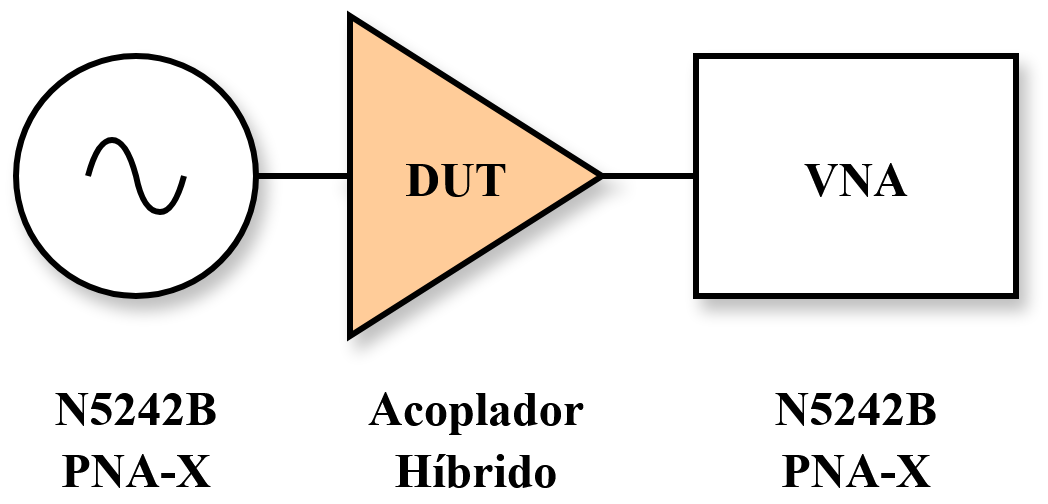
\includegraphics[width=0.5\linewidth]{Figures/07/blocks_coupler.png}
    \caption{Diagrama en bloques del setup de medición de parámetros dispersión del acoplador.}
    \label{fig:setup_medicion_acoplador}
\end{figure}

\subsection{Mediciones del amplificador}
Para validar experimentalmente el diseño propuesto del amplificador, se llevó a cabo un conjunto de mediciones que abarcan el comportamiento de pequeña señal, el desempeño de potencia en gran señal y la caracterización no lineal del dispositivo.

% -----------------------------------------------------------------------------------------------%
\subsubsection{Medición de parámetros dispersión}
Los parámetros de dispersión se midieron con el objetivo de validar el diseño de las redes de adaptación y caracterizar el comportamiento de pequeña señal del amplificador. Se empleó el mismo PNA-X que para las mediciones del acoplador, calibrado mediante el método TOSM con un kit de calibración Keysight 85052B~\cite{calkit}. En el puerto de salida se insertaron en cascada un atenuador de 20\,dB y otro de 10\,dB con el fin de proteger el receptor del VNA frente a los niveles de potencia elevados presentes a la salida del amplificador. En consecuencia, únicamente se reportan los parámetros $S_{21}$ y $S_{11}$, dado que la presencia del atenuador en el puerto de salida impide una medición confiable de los parámetros que involucran la reflexión hacia dicho puerto. El valor medido de $S_{21}$ fue corregido sumando el valor nominal del atenuador.

\begin{figure}[H]
    \centering
    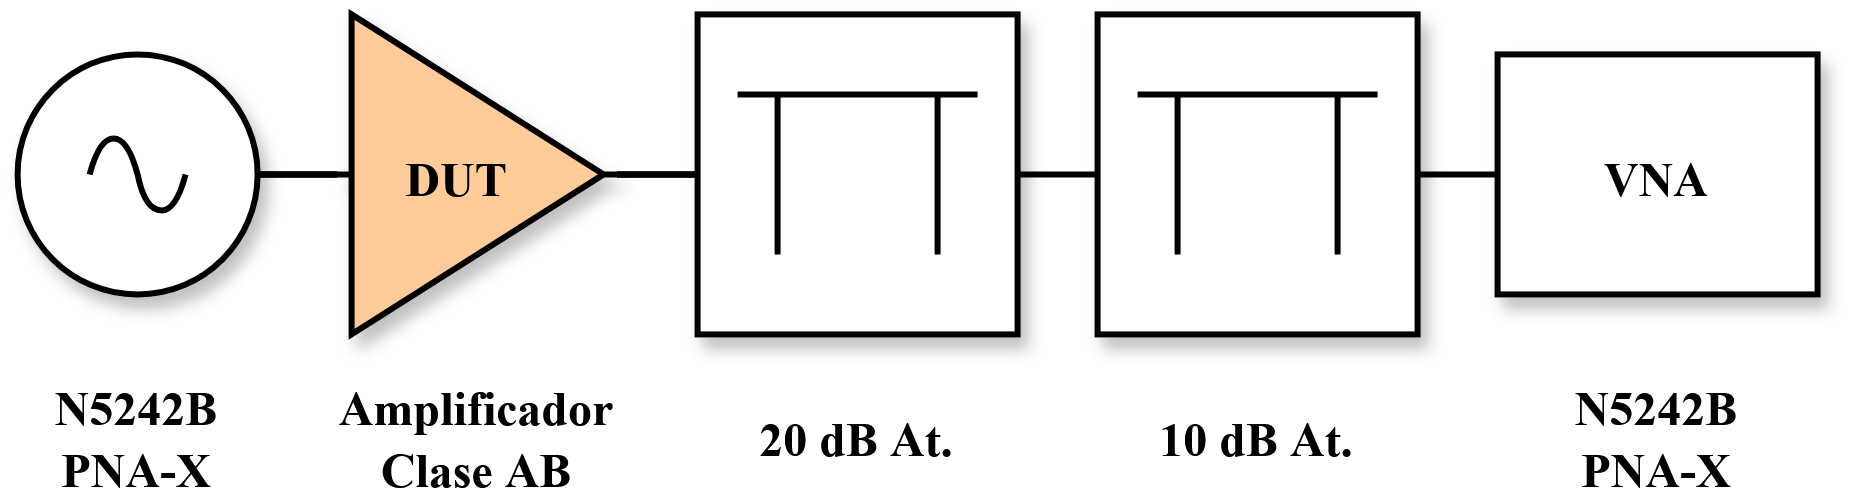
\includegraphics[width=0.8\linewidth]{Figures/07/blocks_sparams.png}
    \caption{Diagrama en bloques del setup de medición de parámetros dispersión del amplificador.}
    \label{fig:setup_medicion_sparam_amp}
\end{figure}

% -----------------------------------------------------------------------------------------------%
\subsubsection{Medición de potencia de salida}
Se realizó una medición de potencia de salida con el fin de caracterizar el comportamiento de gran señal del amplificador. Dado que el dispositivo bajo prueba requiere niveles de excitación superiores a la potencia de salida que el VNA es capaz de entregar, se insertó un amplificador driver Mini-Circuits ZX60-83LN12+~\cite{preamp} entre la fuente de señal del Keysight N5242B y el amplificador de potencia bajo prueba. La potencia de salida se midió con un sensor de potencia Keysight U8485A~\cite{powersensor}, precedido por un atenuador de 20\,dB y un atenuador de 10\,dB. La potencia de entrada se barrió en pasos de 2,5\,dBm a la frecuencia nominal de operación de 2,2\,GHz. A partir de los valores de potencia de entrada y de salida obtenidos mediante este barrido, junto con la medición de la corriente de polarización de drain, se determinaron la ganancia, el punto de compresión de 1\,dB, la potencia de saturación (Psat), la eficiencia de drain y la eficiencia de agregado de potencia (PAE) del amplificador.

\begin{figure}[H]
    \centering
    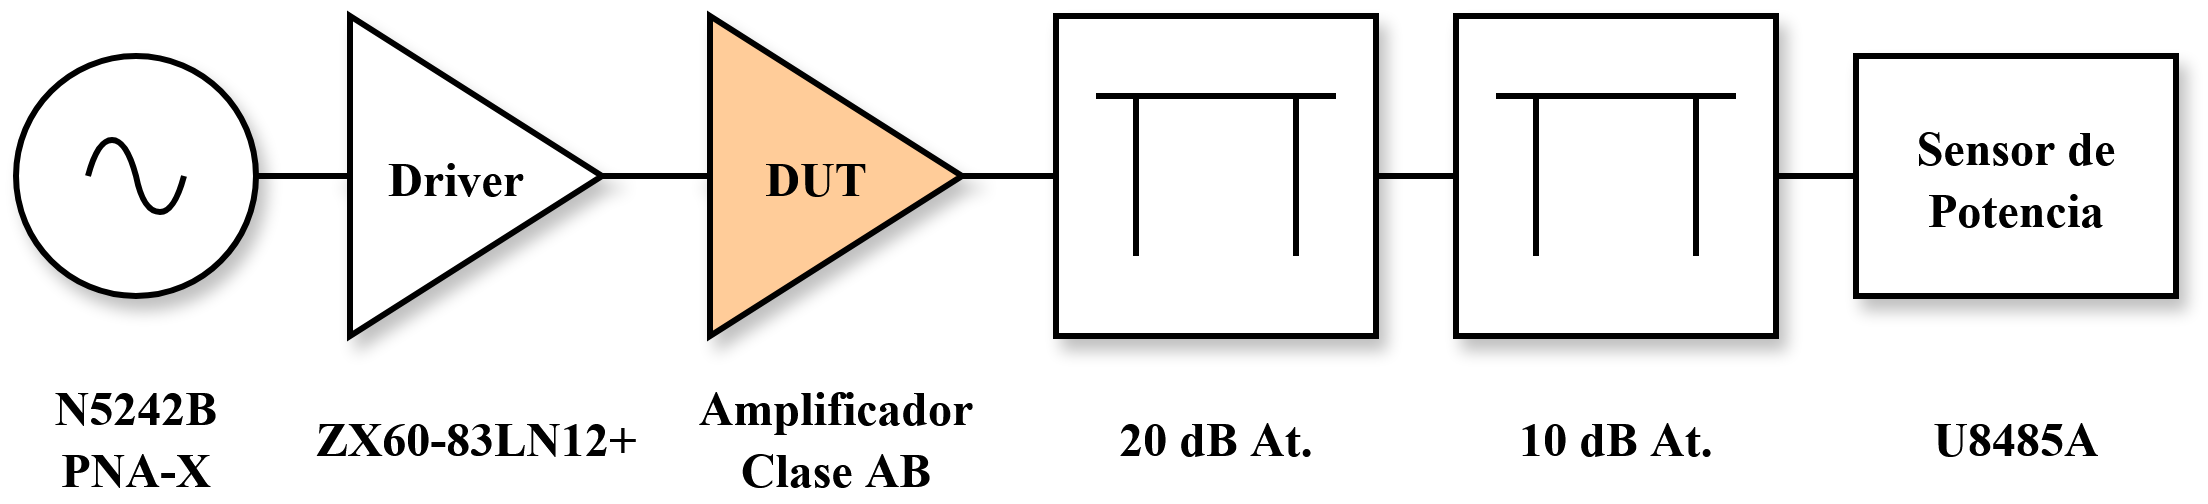
\includegraphics[width=\linewidth]{Figures/07/blocks_p1db.png}
    \caption{Diagrama en bloques del setup de medición de potencia de salida del amplificador.}
    \label{fig:setup_medicion_pout}
\end{figure}

Dado que el amplificador driver ingresa en compresión dentro del rango de medición, el punto de compresión de 1\,dB del dispositivo bajo prueba no puede obtenerse de forma directa a partir de la curva de potencia de salida medida. Por este motivo, se aplicó la expresión de compresión en cascada de la ecuación~\eqref{eq:p1db_cascada}, que refiere la compresión de cada etapa a la entrada del sistema y combina sus contribuciones ponderadas inversamente por la ganancia de las etapas precedentes

\begin{equation}
    \frac{1}{P_{1dB\,sys}} = \frac{1}{G_2 \cdots G_N \, P_{1dB,1}} + \frac{1}{G_3 \cdots G_N \, P_{1dB,2}} + \cdots + \frac{1}{P_{1dB,N}}
    \label{eq:p1db_cascada}
\end{equation}

% -----------------------------------------------------------------------------------------------%
\subsubsection{Medición de distorsión armónica}
Debido a la no linealidad intrínseca de todo dispositivo activo, sumada a la clase de operación en la que se polariza el amplificador, las etapas de potencia generan distorsión armónica que degrada la pureza espectral de la señal y puede provocar interferencia fuera de banda. Para caracterizar este comportamiento, se midieron el segundo y el tercer armónico utilizando un generador de señal Siglent SSG3032X-IQE~\cite{rfgen} como fuente de excitación de onda continua a 2,2\,GHz y un analizador de espectro Keysight N9322C~\cite{spectrumanalyzer} a la salida. Se colocó un atenuador de 20\,dB en la entrada del analizador con fines de protección. La potencia de entrada se barrió desde 0\,dBm hasta 20\,dBm en pasos de 5\,dBm.

\begin{figure}[H]
    \centering
    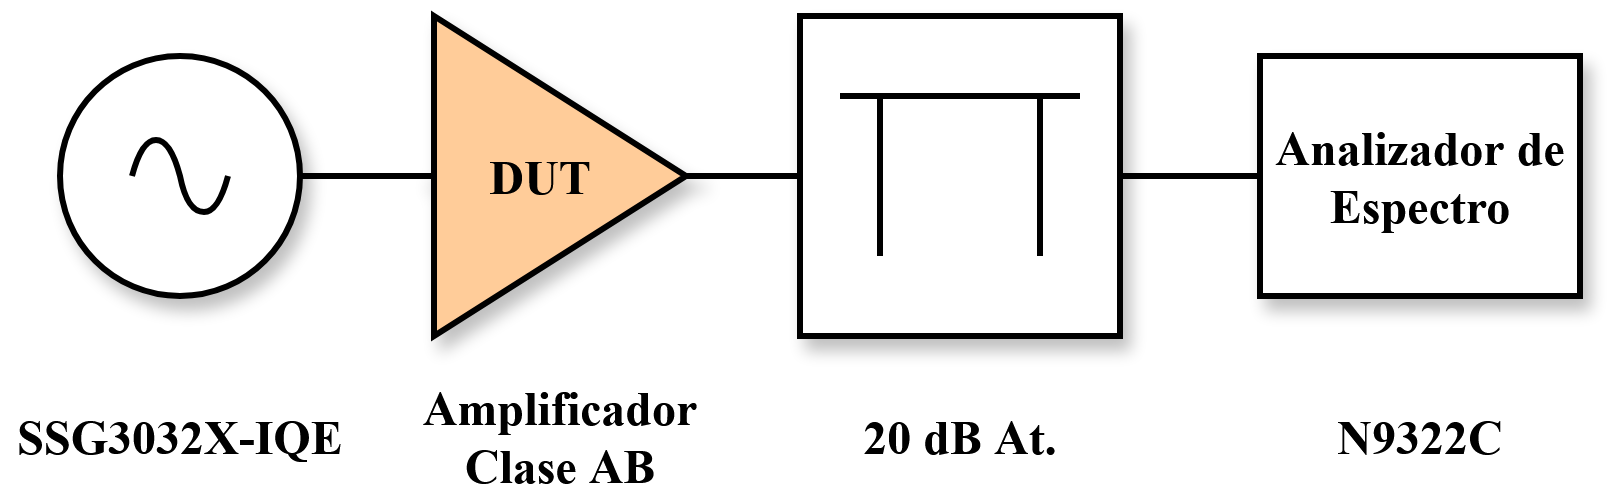
\includegraphics[width=0.7\linewidth]{Figures/07/blocks_harmonic_balance.png}
    \caption{Diagrama en bloques del setup de medición de distorsión armónica del amplificador.}
    \label{fig:setup_medicion_armonicos}
\end{figure}

% -----------------------------------------------------------------------------------------------%
\subsubsection{Medición de OIP3}
Siguiendo el principio de la prueba de dos tonos descripta en la Sección~\ref{sec:dos_tonos}, el punto de intercepción de tercer orden a la salida (OIP3) se obtuvo mediante la aplicación de software ``IMD Sweep'' (S93087B IMD) del VNA Keysight N5242B PNA-X. De forma análoga a la medición de potencia de salida, se incorporó el amplificador driver Mini-Circuits ZX60-83LN12+ entre la fuente de señal del VNA y el dispositivo bajo prueba, con el fin de capturar adecuadamente los efectos de gran señal. Asimismo, se agregaron dos atenuadores de 20\,dB y 10\,dB a la salida del dispositivo bajo prueba para proteger los puertos del VNA. La separación de frecuencia entre los dos tonos se fijó en 10\,MHz, con una potencia de cada tono de $P_{in}=-5\,\text{dBm}$.

\begin{figure}[H]
    \centering
    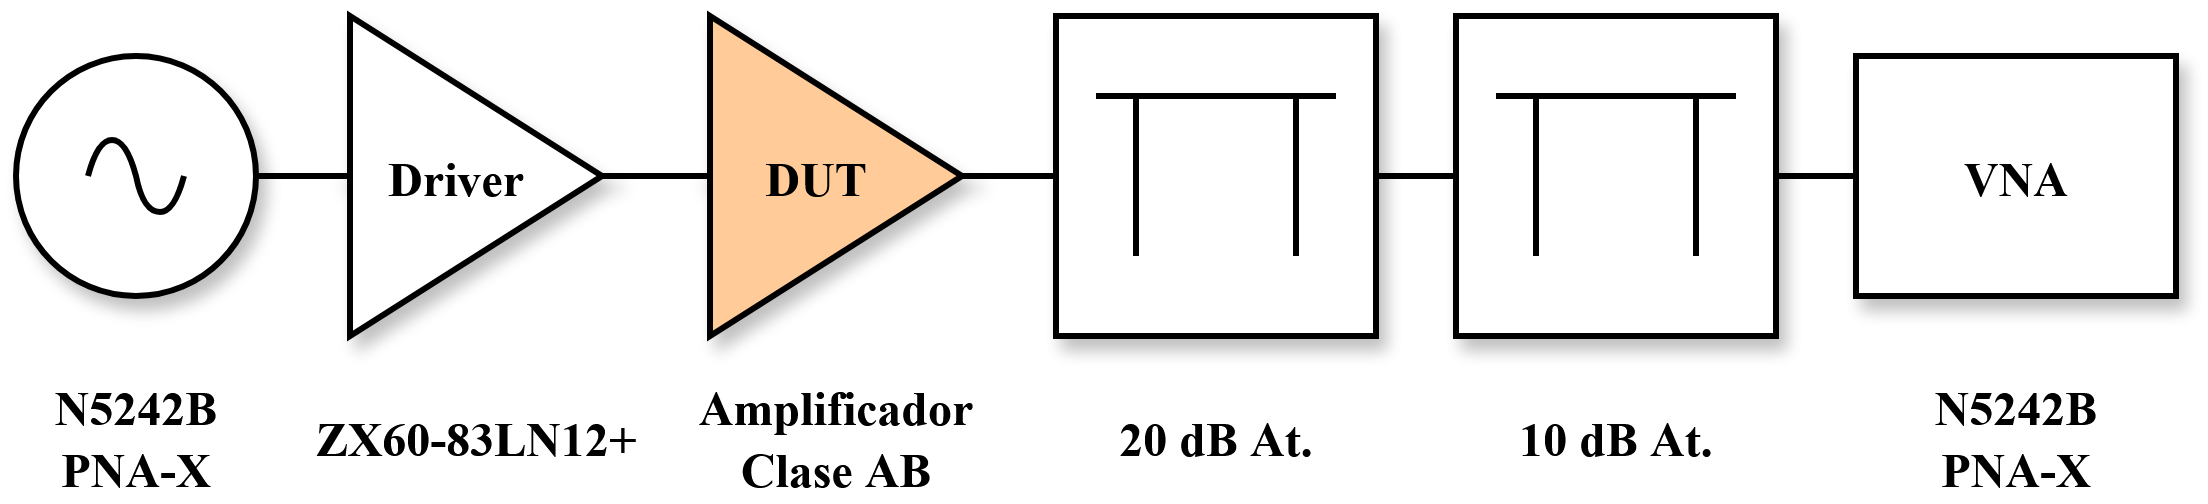
\includegraphics[width=\linewidth]{Figures/07/blocks_oip3.png}
    \caption{Diagrama en bloques del setup de medición de OIP3 del amplificador.}
    \label{fig:setup_medicion_oip3}
\end{figure}